\documentclass[german,ignorenonframetext
,hideothersubsections %% Im Sidebar nur die aktuellen Subsections anzeigen
]{beamer}

\usepackage[ngerman]{babel} % f�r deutsche Spracheinstellungen
\usepackage{graphics} % um Bilder einbinden zu k�nnen
\usepackage[dvips]{epsfig} % um Bilder zu skalieren
\usepackage[applemac]{inputenc} % inputencoding (MacOS) f�r Umlaute und Akzente
\usepackage{multimedia}

%%%%%%%%%%%%%%%%%%%%%%%%%%%%%%%%%%%%%%%%%%%

%%%%%%% Die folgenden Befehle definieren das Grundlayout, blenden auf der
%%%%%%% Titelseite die HAW-Infos ein und setzen das 
%%%%%%% HAW-Logo in die Ecke
\mode<presentation>{\usetheme{Berkeley}}
\logo{\pgfimage[height=1.5cm]{HAW_wuerfel+}}
\institute[MT -- HAW Hamburg]{HAW Hamburg\\ Dept.\ Informatik}

%%%%%%% der folgende Befehl l�sst die mit "\pause" verdeckten Teile der Folien 
%%%%%%% transparent erscheinen.  
\setbeamercovered{transparent}  

%%%%%%% die folgende Sequenz blendet mit jeder neuen Section einmal das 
%%%%%%% Inhaltsverzeichnis mit dem Titel "�bersicht" ein und markiert den
%%%%%%% jeweils aktuellen Gliederungspunkt
\AtBeginSection[]{
\begin{frame}<beamer>
\frametitle{�bersicht} 
\tableofcontents[currentsection,currentsubsection]
\end{frame}
}

%%%%%%%%%%%%%%%%%%%%%%%%%%%%%%%%%%%%%%%%%%%

%%%%%%% jeder dieser Titelseiten-Befehle kennt eine in eckige Klammern gesetzte 
%%%%%%% Kurzform, die im Rand benutzt wird
\title[Interaktive Schnittstellen]{Interaktive Schnittstellen zu virtuellen Welten}
\subtitle{Projekt im Wintersemester 2013}
\author[]{}
\date{\today}

%%%%%%%%%%%%%%%%%%%%%%%%%%%%%%%%%%%%%%%%%%%

\begin{document}

%%%%%% dieser Befehl erzeugt das Deckblatt. 
%%%%%% Mit der Option plain wird das Layout f�r das Deckblatt abgeschaltet
%\frame[plain]{\titlepage}
\frame{\titlepage}

\begin{frame}
  \frametitle{�bersicht}
  \tableofcontents
\end{frame}

%%%%%%%%%%%%%%%%%%%%%%%%%%%%%%%%%%%%%%%%%%%
%%%%%%%%%%%%%%%%%%%%%%%%%%%%%%%%%%%%%%%%%%%
\section{Hardware} 
%%%%%%%%%%%%%%%%%%%%%%%%%%%%%%%%%%%%%%%%%%%
%%%%%%%%%%%%%%%%%%%%%%%%%%%%%%%%%%%%%%%%%%%

\begin{frame}
\frametitle{Emotiv EEG}

\begin{center}  
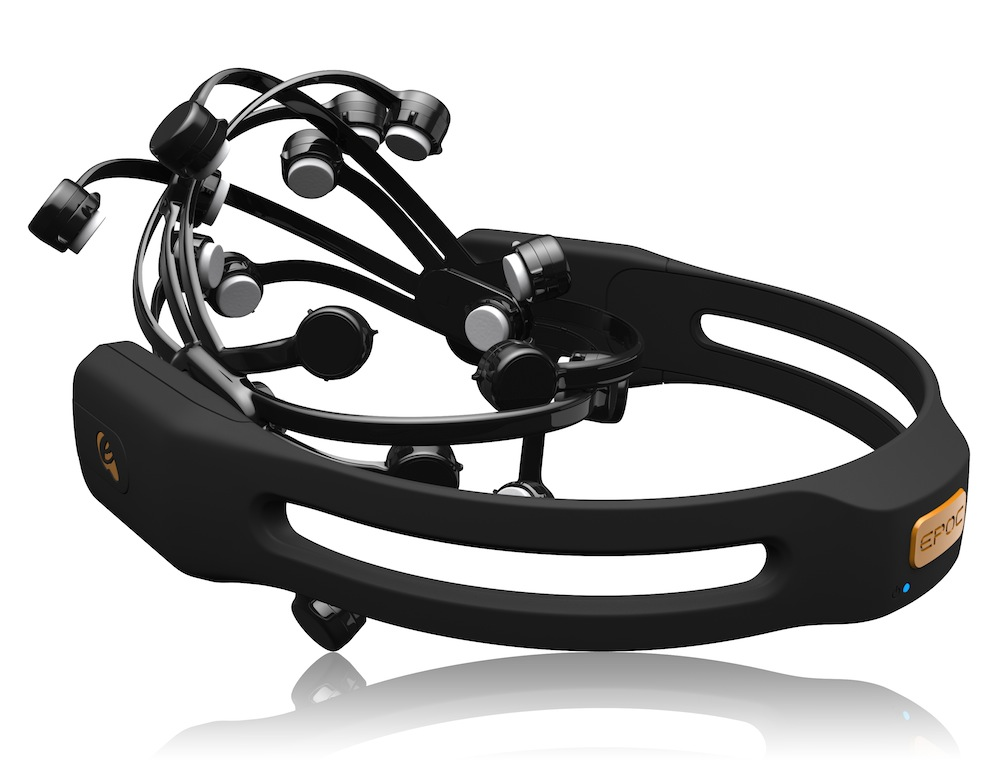
\includegraphics[width=.7\textwidth]{EmotivEEG.jpg}
\end{center}  

\end{frame}


\begin{frame}
  \frametitle{Emotiv-API}
  
  \pgfimage[width=\textwidth]{EmoEngine}
  

\end{frame}

\begin{frame}
  \frametitle{Emotiv-API}
  
  Die Emotiv-API (drei C-Header und entsprechende Binaries) bietet Zugriff auf Daten auf vier veschiedenen Ebenen:
  
\begin{enumerate}
\item rohe Messwerte der 14 Elektroden und des Gyroskops
\item Mimik-Ereignisse (''Expressiv Suite'')
\item ''Emotions-Werte'' (''Affectiv Suite'')
\item trainierte, wiedererkannte ''Gedanken''-Muster (''Cognitiv Suite'')
\end{enumerate} 

Wie die Daten der Ebenen 2-4 berechnet werden, bleibt leider ein Geheimnis der Hersteller-Firma.

\end{frame}

%%%%%%%%%%%%%%%%%%%%%%%%%%%%%%%%%%%%%%%%%%%
%\section{Hardware}
%%%%%%%%%%%%%%%%%%%%%%%%%%%%%%%%%%%%%%%%%%%
\begin{frame}
\frametitle{Neurosky Mindwave}

Das Neurosky BCI ist ein 1-Kanal EEG-Headset.
Erfasst Entspannung- und Aufmerksamkeit auf Basis von EEG-Messungen.
 

\begin{figure}
	\centering
		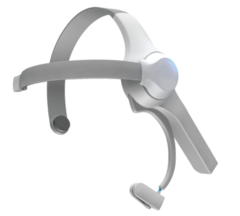
\includegraphics[scale=0.50]{MindWave.png}
	\caption{Neurosky-Mindwave}
	\label{fig:MindWave}
\end{figure}

\end{frame}


\begin{frame}
\frametitle{Microsoft Kinect}
Die Kinect ist ein Sensor f�r Bilderfassung.\\
Der Tiefensensor, hat einen IR-Laserprojektor sowie ein CMOS Monochrom-Kameramodul.

\begin{figure}
	\centering
		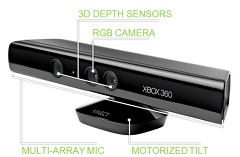
\includegraphics[scale=0.70]{KinectSensor}
	\caption{Microsoft-Kinect}
	\label{fig:KinectSensor}
\end{figure}


\end{frame}

%%%%%%%%%%%%%%%%%%%%%%%%%%%%%%%%%%%%%%%%%%%
%%%%%%%%%%%%%%%%%%%%%%%%%%%%%%%%%%%%%%%%%%%
\section{Signalanalyse} 
%%%%%%%%%%%%%%%%%%%%%%%%%%%%%%%%%%%%%%%%%%%
%%%%%%%%%%%%%%%%%%%%%%%%%%%%%%%%%%%%%%%%%%%



%%%%%%%%%%%%%%%%%%%%%%%%%%%%%%%%%%%%%%%%%%%
%\section{Datenanalyse} 
%%%%%%%%%%%%%%%%%%%%%%%%%%%%%%%%%%%%%%%%%%%

\begin{frame}
\frametitle{Video ''linkes Bein''}
\movie[externalviewer]{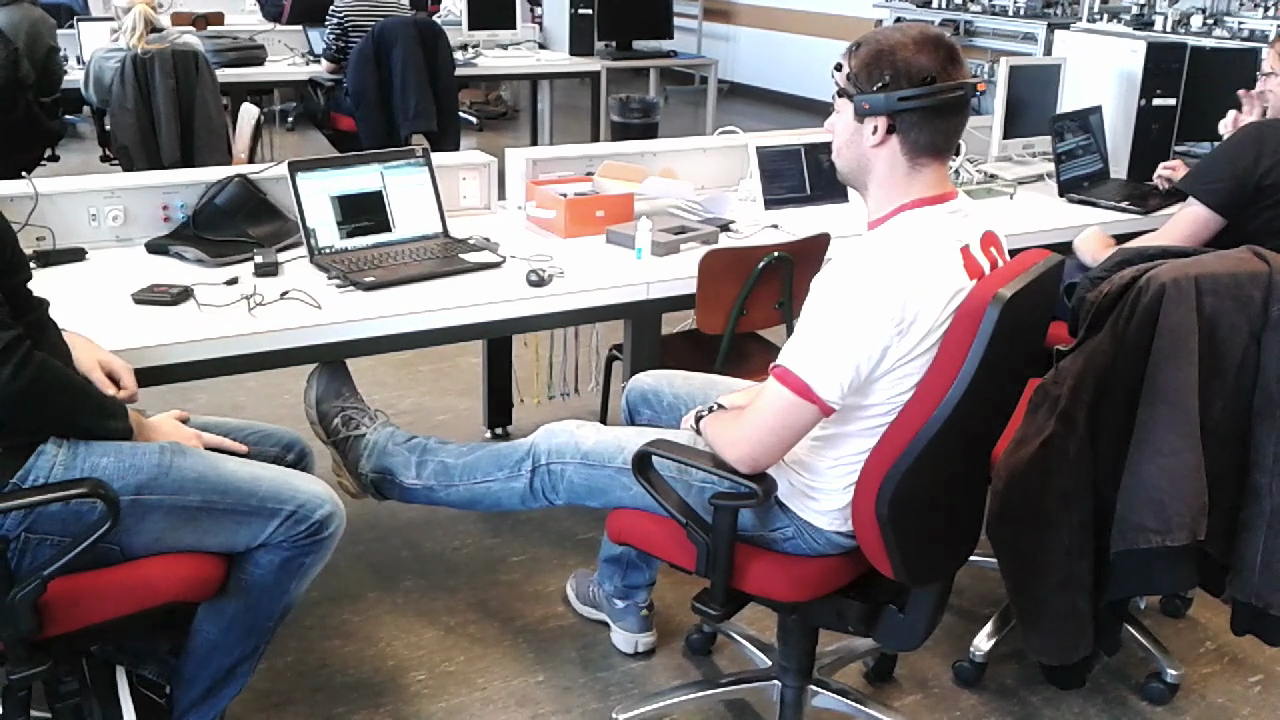
\includegraphics[width=\textwidth]{Snapshot_linkes_Bein.png}} {Video_linkes_Bein_edit.mov} %% Snapshot �ndern!!!!
\end{frame}

\begin{frame}
\frametitle{Auswertung - erste Versuche}
  
\pgfimage[width=\textwidth]{linplot_linkes_bein.png}
  
\end{frame}

\begin{frame}
\frametitle{Auswertung - mit bwview}
 
\begin{center}  
\pgfimage[width=\textwidth]{Video_linkes_Bein_bfview.png}
\end{center}  
\end{frame}

%%%%%%%%%%%%%%%%%%%%%%%%%%%%%%%%%%%%%%%%%%%
%\section{Datenanalye Frequenzb�nder und Sensorregionen}
%%%%%%%%%%%%%%%%%%%%%%%%%%%%%%%%%%%%%%%%%%%

\begin{frame}
  \frametitle{Analyse der EEG-Rohdaten mit Fokus auf Kognitive Belastung}
  
  \pgfimage[width=0.7\textwidth]{CognitiveAreas.png}
  

\end{frame}

\begin{frame}
  \frametitle{Analyse der EEG-Rohdaten mit Fokus auf Kognitive Belastung}
  
  \pgfimage[width=0.7\textwidth]{GaussScalingSensors.png}
  

\end{frame}

\begin{frame}
  \frametitle{Auswahl eines geeigneten Datensatzes}
  
  \pgfimage[width=0.7\textwidth]{eegSignals3D.png}
  

\end{frame}

\begin{frame}
  \frametitle{Betrachtung des Frequenzspektrums}
  
  \pgfimage[width=0.7\textwidth]{SpectrogramSpatialResult.png}
  

\end{frame}

\begin{frame}
  \frametitle{Betrachtung des Frequenzspektrums}
  
  \pgfimage[width=0.7\textwidth]{SpectrogramSpatialResultZoom.png}
  

\end{frame}

\begin{frame}
  \frametitle{Thetabandanalyse}
  \begin{itemize}
  \item Anwendung der Gewichtungsfaktoren
  \item Zusammensetzen des raeumlichen Signals
  \item Bandpassfilterung mit Durchlassbereich von 4 bis 7,5 Hz
  \item Betrachtung der Energiedichte
  \end{itemize}
  
  
  
  \pgfimage[width=0.7\textwidth]{spatialcognitivedata.png}
  

\end{frame}


%%%%%%%%%%%%%%%%%%%%%%%%%%%%%%%%%%%%%%%%%%%
%%%%%%%%%%%%%%%%%%%%%%%%%%%%%%%%%%%%%%%%%%%
\section{Hardware-Abstraktions-Layer} 
%%%%%%%%%%%%%%%%%%%%%%%%%%%%%%%%%%%%%%%%%%%
%%%%%%%%%%%%%%%%%%%%%%%%%%%%%%%%%%%%%%%%%%%


%%%%%%%%%%%%%%%%%%%%%%%%%%%%%%%%%%%%%%%%%%%
\subsection{Emotiv Epoc API Wrapper} % die sections sind hier nur zum Strukturieren des Vortrags!!
%% der Name der section taucht nur im Inhaltsverzeichnis und im linken Rand auf.
%%%%%%%%%%%%%%%%%%%%%%%%%%%%%%%%%%%%%%%%%%%

\begin{frame}
  \frametitle{Emotiv Epoc API}
  
Die Emotiv Epoc API ist nativ in C geschrieben.
Sie ist dabei jedoch umst�ndlich, und nur m��ig dokumentiert.
\linebreak
Deswegen: Entwicklung eines Wrappers f�r eine komfortablere Nutzung des EEG Headsets.

\end{frame}

\begin{frame}
  \frametitle{Emotiv Epoc API Wrapper}
  
Der API Wrapper ist in C++ geschrieben.
Bei der Entwicklung wurde auf objektorientierte Prinzipien geachtet.
Es wurde ebenfalls eine allgemeine Schnittstelle definiert, die es erm�glicht mit minimalem Aufwand unterschiedliche EEG Headsets zu nutzen

\end{frame}


%%%%%%%%%%%%%%%%%%%%%%%%%%%%%%%%%%%%%%%%%%%
\subsection{Verteilte Systeme mit OSC-Kopplung}
%%%%%%%%%%%%%%%%%%%%%%%%%%%%%%%%%%%%%%%%%%%

\begin{frame}
  \frametitle{Verteilte Systeme mit OSC-Kopplung}
  
  \pgfimage[width=\textwidth]{ServerComponents}
  

\end{frame}

\begin{frame}
  \frametitle{OSC Server}
  
  \pgfimage[width=\textwidth]{OSC_Server}
  

\end{frame}

\begin{frame}
  \frametitle{Message Thread}
  
  \pgfimage[width=\textwidth]{Message_Thread}
  

\end{frame}

\begin{frame}
  \frametitle{OSC}
  
  Wieso Open Sound Control Nachrichten:
  
\begin{enumerate}
\item Plattform- und Sprachunabh�ngig
\item die asynchrone Kommunikation verhindert Deadlocks
\item einfacher Aufbau der Nachrichten
\item f�r die meisten Sprachen gibt es Open Source Implementierungen
\end{enumerate} 

\end{frame}

%%%%%%%%%%%%%%%%%%%%%%%%%%%%%%%%%%%%%%%%%%%
%%%%%%%%%%%%%%%%%%%%%%%%%%%%%%%%%%%%%%%%%%%
\section{Anwendungen} 
%%%%%%%%%%%%%%%%%%%%%%%%%%%%%%%%%%%%%%%%%%%
%%%%%%%%%%%%%%%%%%%%%%%%%%%%%%%%%%%%%%%%%%%


%%%%%%%%%%%%%%%%%%%%%%%%%%%%%%%%%%%%%%%%%%%
\subsection{Torcs} % die sections sind hier nur zum Strukturieren des Vortrags!!
%% der Name der section taucht nur im Inhaltsverzeichnis und im linken Rand auf.
%%%%%%%%%%%%%%%%%%%%%%%%%%%%%%%%%%%%%%%%%%%

\begin{frame}
\frametitle{Torcs - The Open Racing Car Simulator}

\begin{center}
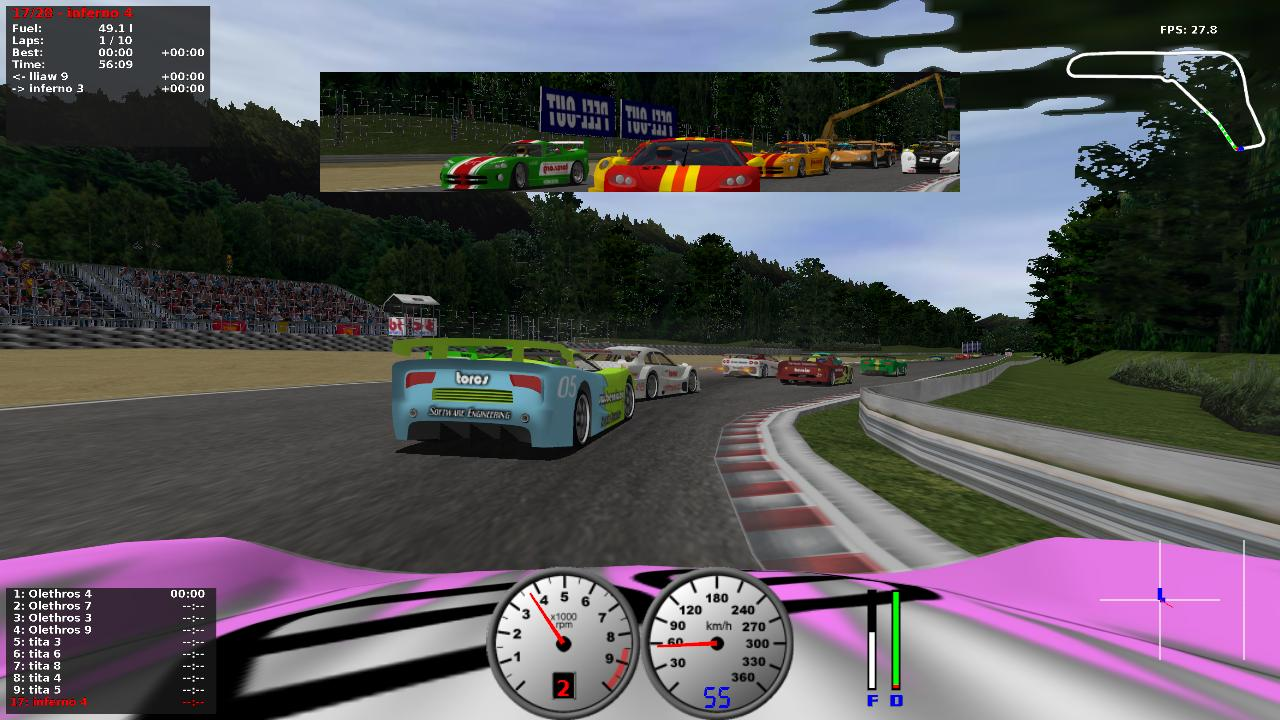
\includegraphics[width=\textwidth]{torcs-screenshot.png}
\end{center}
\end{frame}


\begin{frame}
\frametitle{Torcs - The Open Racing Car Simulator}

%%%%% AUSSCHNEIDEN


\begin{itemize}
\item Open Source Lizenz - GPL
\item 3D Rennspiel
\item Fahrer programmierbar
\item Gangschaltung per EEG
\item http://torcs.sourceforge.net/
\end{itemize}
\end{frame}


\begin{frame}
\frametitle{Interaktion}
\begin{center}
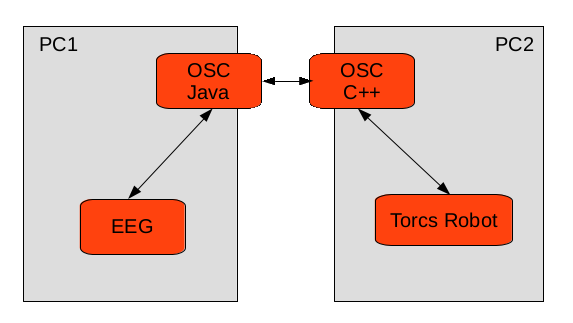
\includegraphics[scale=0.5]{torcs.png}
\end{center}
\end{frame}


%%%%%%%%%%%%%%%%%%%%%%%%%%%%%%%%%%%%%%%%%%%
\subsection{Komposition f�r ein EEG}
%%%%%%%%%%%%%%%%%%%%%%%%%%%%%%%%%%%%%%%%%%%

\begin{frame}
\frametitle{Kooperation mit der HMTM Hannover}       
\begin{center}  
\pgfimage[width=.9\textwidth]{Hochschule_fuer_Musik_und_Theater_Hannover.jpg}

Hochschule f�r Musik, Theater und Medien Hannover
\end{center}  

\end{frame}

%%%%%%%%%%%%%%%%%%%%%%%%%%%%%%%%%%%%%%%%%%%
\subsection{Abstrakte Kunst}
%%%%%%%%%%%%%%%%%%%%%%%%%%%%%%%%%%%%%%%%%%%
\begin{frame}

\frametitle{Mit den H�nden malen und mit den Gedanken f�rben}       

%\begin{columns}
%\column{.4\textwidth}
%\begin{center}
%\pgfimage[height = 1\textwidth]{code} \\
%\scriptsize
%	Abstrakte Kunst
%\end{center}
%\end{columns}

\begin{figure}
	\centering
		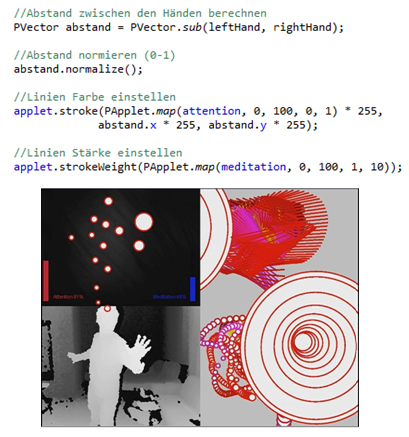
\includegraphics[width=0.60\textwidth]{code.PNG}
	\caption{Abstrakte Kunst}
	\label{fig:code}
\end{figure}



\end{frame}


%%%%%%%%%%%%%%%%%%%%%%%%%%%%%%%%%%%%%%%%%%%
\subsection{Audio Aufnahme und Steuerung von Gitarreneffekten}
%%%%%%%%%%%%%%%%%%%%%%%%%%%%%%%%%%%%%%%%%%%


\begin{frame}

\frametitle{Playing Music}


\begin{figure}
	\centering
		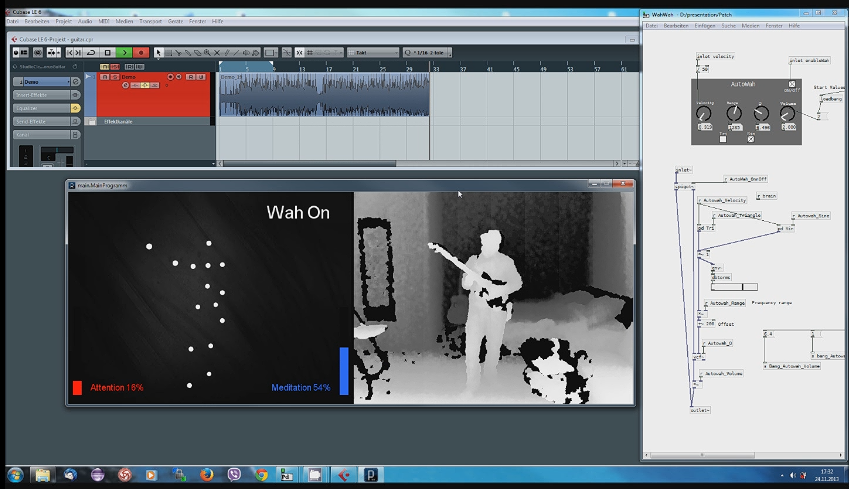
\includegraphics[scale=0.4]{Audio.PNG}
	\caption{schnappschuss aus dem Video [Carlos Santana-Europa(cover)]}
	\label{fig:Audio}
\end{figure}




\end{frame}



\end{document} %%%%% END DOCUMENT %%%%%%


%%%%%%%%%%%%%%%%%%%%%%%%%%%%%%%%%%%%%%%%%%%
%%  besondere Gestaltungselemente f�r Vortragsfolien
%%%%%%%%%%%%%%%%%%%%%%%%%%%%%%%%%%%%%%%%%%%

% Folie
\begin{frame}
\frametitle{Folientitel}
        Text, Bilder, Bl�cke
\end{frame}

% neutraler Kasten
\begin{block}{Blocktitel}
        Blocktext
\end{block}

% gr�ner Kasten
\begin{exampleblock}{Beispielblocktitel}
        Beispielblocktext
\end{exampleblock}

% roter Kasten
\begin{alertblock}{Warnungsblocktitel}
        Warnungsblocktext
\end{alertblock}

% mehrspaltige Folie mit variablen Spaltenbreiten
\begin{columns}
\column{.55\textwidth}
        Text oder Bild
\column{.45\textwidth}
        Text oder Bild
\end{columns}

% sukzessiver Folienaufbau 
\pause

% mehr Befehle f�r sukzessiven Folienaufbau, 
% der geklammerte Teil erscheint jeweils ab der dritten Teil-Folie
\uncover<3->{}
\only<3->{}
\invisible<1-2>{}

% rote Markierung des geklammerten Teils bei der vierten Teil-Folie
\alert<4>{}

%%%%%%%%%%%%%%%%%%%%%%%%%%%%%%%%%%%%%%%%%%%